\documentclass[fleqn,11pt]{article}

% __________________________________________________________ PACKAGES AND DEFINITIONS
% ___________________________________________________________________________________

% Numbering of sections and subsections
\setcounter{secnumdepth}{3}

% This avoids redundancy in math alphabets
\newcommand{\bmmax}{0}

\usepackage[a4paper, total={160mm,240mm}]{geometry}
\usepackage{amsfonts, amsmath, bm}
\usepackage{setspace}
\usepackage{subcaption}
\usepackage[font=footnotesize]{caption}
\captionsetup[table]{skip=0pt}

% tikz
\usepackage{tikz}
\usepackage{pgfplots}
\pgfplotsset{compat=1.17}

% Avoid re-drawing unchanged tikz figures
\usetikzlibrary{external}
\tikzexternalize

% Bibliography style
\bibliographystyle{spmpsci}

% Font
\renewcommand*\rmdefault{bch}

% Spacing
\setstretch{1.5}
\renewcommand{\arraystretch}{1.136}
\setlength{\parskip}{1em}				% Separation between paragraphs
\frenchspacing

% Spacing before section titles
\usepackage{titlesec}
%\titlespacing*{<command>}{<left>}{<before-sep>}{<after-sep>}
\titlespacing*{\section}
{0pt}{8ex plus 1ex minus .2ex}{0.3ex plus .2ex minus .2ex}
\titlespacing*{\subsection}
{0pt}{7ex plus 1ex minus .2ex}{0.3ex plus .2ex minus .2ex}

\setlength{\skip\footins}{1cm}

% Headers
\usepackage{fancyhdr}
\pagestyle{fancy}
\setlength\headheight{26pt}
\renewcommand{\footrulewidth}{0.4pt}% default is 0pt

% This one is needed to avoid two "REFERENCES" header in the bibliography pages
\fancypagestyle{bib}{
	\fancyhf{}
	\fancyhead[LE,RO]{%
		% We want italics
		\itshape
		% The chapter title
		\leftmark}
	\fancyfoot[C]{\thepage}
}


% Empty page at the end of a section
\def\blankpage{%
	\clearpage%
	\thispagestyle{empty}%
	\addtocounter{page}{-1}%
	\null%
	\clearpage}

% ____________________________________________________________________________ MACROS
% ___________________________________________________________________________________

\definecolor{brick_red}		{RGB}{128,0,0}
\definecolor{dark_blue}		{RGB}{75,120,50}
\definecolor{bright_blue}	{RGB}{0,0,200}
\definecolor{dark_green}	{RGB}{0,128,0}
\definecolor{black}			{RGB}{0,0,0}
\definecolor{orange}		{RGB}{255,94,19}

% Parentheses
\newcommand{\plbr}[1]		{ \left( #1 \right) }
\newcommand{\sqbr}[1]		{ \left[ #1 \right] }
\newcommand{\cubr}[1]		{ \left\{ #1 \right\} }

% Matrices and vectors
\newcommand{\cvvect}[1]		{ \begin{array}{c} #1 \end{array} }
\newcommand{\hvect}[2]		{ \begin{array}{ #1 } #2 \end{array} }
\newcommand{\matr}[2]		{ \begin{array}{ #1 } #2 \end{array} }

\newcommand{\mat}[2]		{ \sqbr{\begin{array}{ #1 } #2 \end{array}} }

% Operations
\newcommand{\trans}			{^{\rm T}}
\newcommand{\eq}			{ \; = \; }

% Variables
\newcommand{\timestep}		{ {h} }

% Units
\newcommand{\unit}[1]		{ {\; \rm #1} }

% ___________________________________________________________________________________
% ___________________________________________________________________________________

\begin{document}
	
	\vspace{1cm}
	
	\title{\LARGE \bf Co-simulation benchmarks: Linear oscillator}
	
	\author{\\ \bf Laboratorio de Ingenier\'ia Mec\'anica - LIM \\ \bf Universidade da Coru\~na}
	
	\maketitle
	
	{\let\newpage\relax\maketitle}
	{\thispagestyle{fancy}
		\fancyfoot[C]{}
		\lhead{
\includegraphics[width=1.24cm]{./fig/LIM-logo.pdf}}
		\rhead{
\includegraphics[width=3.4cm]{./fig/cosimbauto-logo.pdf}}}
	
	\newpage
	
	\fancyhf{}
	\pagestyle{fancy}
	\fancyhead[L]{\ifodd\value{page}\else
		Linear oscillator \fi}
	\fancyhead[C]{\ifodd\value{page} \fi}
	\fancyhead[R]{\ifodd\value{page} Benchmark problem \fi}
	\fancyfoot[C]{\thepage}
	
% ___________________________________________________________________________________

\textit{
	This document describes a classical benchmark in the co-simulation literature: a two degree-of-freedom linear oscillator.
}
	
\textit{
	Contact Francisco Gonz\'alez (f.gonzalez@udc.es) if you have questions or comments about this example. 
}

% ___________________________________________________________________________________
\section{Problem description}
\label{ProblemDefinition}

This problem consists in a two-degree-of-freedom linear oscillator, shown in Fig.~\ref{fig:LinearOscillator}, composed by two masses $m_1$ and $m_2$ connected to each other and to the ground by means of linear springs and dampers.
Variables $x_1$ and $x_2$ measure the displacement of each mass with respect to its equilibrium position, in which all the spring forces are zero.
The initial position and velocity of each mass are denoted by $x_{i,0}$ and $\dot{x}_{i,0}$, respectively, with $i=1,2$.
Similar systems have been employed as benchmark problems in the co-simulation literature, e.g., \cite{Gonzalez2019, Gonzalez2011, Sadjina2017, Schweizer2015, Schweizer2014}.

\begin{figure}[ht]
	\centering
	\begin{tikzpicture}
		% Node Coordinates for text
		
		% Colors
		\definecolor{figureBlue}{RGB}{65,113,156};
		\definecolor{figureRed}{RGB}{192,0,0};
		
		% Figure Drawing
		\node at (0,0) {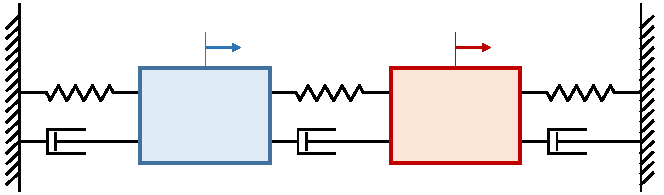
\includegraphics{./fig/LinearOscillator.pdf}};
		
		% Text
		\node[align=center, color = figureBlue] 	at (-21mm, -3.5mm) {$m_1$};
		\node[align=center, color = figureRed] 		at ( 21mm, -3.5mm) {$m_2$};
		\node[align=center, color = figureBlue] 	at (-18mm, 12.5mm) {$x_1$};
		\node[align=center, color = figureRed] 		at (24mm, 12.5mm) {$x_2$};
		
		\node[align=center, color = black] 			at (0mm, 5.5mm) {$k_{\rm c}$};
		\node[align=center, color = black] 			at (0mm, -13.0mm) {$c_{\rm c}$};
		\node[align=center, color = black] 			at (-42mm, 5.5mm) {$k_1$};
		\node[align=center, color = black] 			at (-42mm, -13.0mm) {$c_1$};
		\node[align=center, color = black] 			at (42mm, 5.5mm) {$k_2$};
		\node[align=center, color = black] 			at (42mm, -13.0mm) {$c_2$};
		
	\end{tikzpicture}
	\caption{A two-degree-of-freedom linear oscillator}
	\label{fig:LinearOscillator}
\end{figure}

The linear oscillator problem has a known analytical solution.

% -----------------------------------------------------------------------------------------------
\subsection{Physical properties}
\label{PhysicalProperties}

Different values of the system parameters can be selected to represent a wide range of mechanical systems.
Table~\ref{tab:systemParameters} shows the combinations of parameters used for this benchmark problem in particular.

\begin{table}[ht]
\begin{center}	
	{ \footnotesize{
			\renewcommand{\arraystretch}{1.25}
			\begin{tabular}{lcccccccccccc}
				\hline
				& $m_1$ 	& $m_2$ 	&$k_1$ & $k_{\rm c}$  &$k_2$ &$c_1$ & $c_{\rm c}$ &$c_2$ 
				&$x_{1,0}$ 	&$x_{2,0}$	&$\dot{x}_{1,0}$ 	&$\dot{x}_{2,0}$	\\
				Case	& (kg)		& (kg)	&(N/m) &(N/m) 	&(N/m) &(Ns/m) &(Ns/m) &(Ns/m)  
				& (m) 		& (m)	&(m/s) &(m/s)\\
				\hline
				1	& $1$ 	& $1$ 	& $10$ & $100$ & $1000$ &0 &0 &0 &0 &0 &100 &-100 \\
				2	& $1$ 	& $1$ 	& $10$ & $100$ & $1000$ &$0.01$ &$0.01$ &$0.01$ &0 &0 &100 &-100 \\
				\hline
			\end{tabular}
	}}
\end{center}
\caption{Combinations of system parameters used in this problem}
\label{tab:systemParameters}
\end{table}


% -----------------------------------------------------------------------------------------------
\subsection{Dynamics equations}
\label{DynEquations}

The oscillator dynamics is described by two ordinary differential equations (ODE) that can be expressed in terms of the mass positions ${\bf x} = \sqbr{x_1, x_2}\trans$ and their derivatives with respect to time as
%
\begin{equation}
	{\bf M}\ddot{\bf x} + {\bf C}\dot{\bf x} + {\bf K}{\bf x} \eq {\bf f}
	\label{eq:linearOscillatorDynEqsCompact}
\end{equation}
%
where
%
\begin{equation}
	\matr{ll}
	{
	{\bf M} \eq \sqbr{\matr{cc}{m_1 &0 \\ 0 &m_2}}\,;
	&{\bf C} \eq \sqbr{\matr{cc}{c_1 + c_{\rm c} &-c_{\rm c} \\ -c_{\rm c} &c_2 + c_{\rm c}}} 
	\\
	\\ 
	{\bf K} \eq \sqbr{\matr{cc}{k_1 + k_{\rm c} &-k_{\rm c} \\ -k_{\rm c} &k_2 + k_{\rm c}}}\,;
	& {\bf f} \eq \sqbr{\cvvect{f_1 \\ f_2}} 
	}
	\label{eq:linearOscillatorDynEqsTerms}
\end{equation}
%

If the external forces $\bf f$ are zero, an analytical solution of the dynamics equations~\eqref{eq:linearOscillatorDynEqsCompact} can be found reordering them into the form
\begin{equation}
	\dot{\bf z} = {\bf A}{\bf z}
	\label{eq:linearOscillatorDynEqsLinear}
\end{equation}
where
\begin{align}
	\label{eq:linearOscillatorDynEqsLinearTermsz}
	{\bf z} &\eq \mat{cccc}{x_1 & x_2 & \dot{x}_1 & \dot{x}_2}\trans
	\\
	{\bf A} &\eq \mat{cccc}{
		0 &0 &1 &0 \\ 0 &0 &0 &1 \\
		-\plbr{k_1 + k_{\rm c}}/m_1 &k_{\rm c}/m_1 
		&-\plbr{c_1 + c_{\rm c}}/m_1 &c_{\rm c}/m_1 \\
		k_{\rm c}/m_2 &-\plbr{k_2 + k_{\rm c}}/m_2 
		&c_{\rm c}/m_2 &-\plbr{c_2 + c_{\rm c}}/m_2 }
	\label{eq:linearOscillatorDynEqsLinearTerms}
\end{align}
%
The analytical solution to Eq.~\eqref{eq:linearOscillatorDynEqsLinear} has the form
\begin{equation}
	{\bf z}\plbr{t} \eq e^{\displaystyle{\bf A}\plbr{t-t_0}} \cdot {\bf z}_0
	\label{eq:linearOscillatorDynEqsLinearSol}
\end{equation}

The linear oscillator can also be simulated using a monolithic approach solving the initial value problem defined by Eq.~\eqref{eq:linearOscillatorDynEqsCompact} and the starting system configuration and velocity.
A possibility is using the semi-implicit forward Euler formula as numerical integrator
\begin{equation}
	\dot{\bf x}_{k+1} \eq \dot{\bf x}_{k} + \timestep \ddot{\bf x}_{k}
	\;; \quad\quad\quad\quad
	{\bf x}_{k+1} \eq {\bf x}_{k} + \timestep \dot{\bf x}_{k+1}
	\label{eq:fwEuler}
\end{equation}
where $\timestep$ is the integration step-size.

% _______________________________________________________________________________________________
\section{Subsystem definition}
\label{Schemes}

The oscillator can be decomposed into two subsystems, each of them taking care of the simulation of the dynamics of one of the point masses.
Afterwards, co-simulation can be performed according to many different coupling schemes, e.g., 
Jacobi and Gauss-Seidel configurations, either explicit or implicit, both in single-rate and multi-rate communication grids.
The following selections of coupling variables are put forward for the definition of this benchmark example:
\begin{itemize}
	\item{Force-displacement coupling (\textbf{f-s})} 
	\item{Displacement-displacement coupling (\textbf{s-s}) }
	\item{Force-force coupling (\textbf{f-f}) }
\end{itemize}
%
The selection of coupling variables determines subsystem definition, as shown next.

% -----------------------------------------------------------------------------------------------
\subsection{Force-displacement co-simulation}
\label{ForceDisplacement}

A first option is dividing the oscillator into two subsystems as shown in Fig.~\ref{fig:LinearOscillatorCosim1}.
Subsystem $\mathcal{M}_1$ integrates the dynamics of the first mass and passes the coupling force $f^{\rm c}$ as output to subsystem $\mathcal{M}_2$, which takes care of the second mass and, in turn, delivers its position as output, $\xi^{\rm c}$.

\begin{figure}[ht]
	\centering
	\begin{tikzpicture}
		
		% Colors
		\definecolor{figureBlue}{RGB}{65,113,156};
		\definecolor{figureRed}{RGB}{192,0,0};
		\definecolor{figureGreen}{RGB}{56,87,35};
		
		% Figure Drawing
		\node at (0,0) {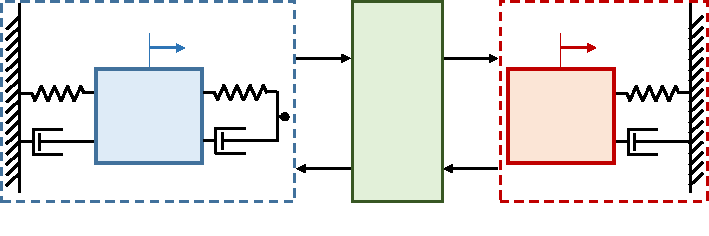
\includegraphics{./fig/LinearOscillatorCosim.pdf}};
		
		% Text
		\node[align=center, color = figureBlue] 	at (-34.5mm, 0mm) {$m_1$};
		\node[align=center, color = figureRed] 		at ( 35mm, 0mm) {$m_2$};
		\node[align=center, color = figureBlue] 	at (-30mm, 14.5mm) {$x_1$};
		\node[align=center, color = figureRed] 		at (40mm, 14.5mm) {$x_2$};
		
		\node[align=center, color = black] 			at (-19mm, 8.5mm) {$k_{\rm c}$};
		\node[align=center, color = black] 			at (-19mm, -8.7mm) {$c_{\rm c}$};
		\node[align=center, color = black] 			at (-50mm, 8.5mm) {$k_1$};
		\node[align=center, color = black] 			at (-50mm, -8.7mm) {$c_1$};
		\node[align=center, color = black] 			at (50mm, 8.5mm) {$k_2$};
		\node[align=center, color = black] 			at (50mm, -8.7mm) {$c_2$};
		
		\node[align=center, color=black] 			at (-5.5mm, 13.5mm) {$f^{\rm c}_1$};
		\node[align=center, color=black] 			at (19.5mm, 13.5mm) {$f^{\rm c}_2$};
		\node[align=center, color=black] 			at (-5.5mm, -13.1mm) {$\xi^{\rm c}_1$};
		\node[align=center, color=black] 			at (19.5mm, -13.1mm) {$\xi^{\rm c}_2$};
		
		\node[align=center, color = figureGreen] 	at (-5mm, 0mm) {$H_1$};
		\node[align=center, color = figureGreen] 	at (19.5mm, 0mm) {$H_2$};
		
		\node[align=center, color = figureBlue] 	at (-34.5mm, -19mm) {Subsystem $\mathcal{M}_1$};
		\node[align=center, color = figureRed] 		at (42.0mm, -19mm) {Subsystem $\mathcal{M}_2$};
		
		\node[align=center, color = figureGreen] 	at (7.5mm, -19mm) {Manager};
		
	\end{tikzpicture}
	\caption{The linear oscillator arranged following a force-displacement coupling scheme}
	\label{fig:LinearOscillatorCosim1}
\end{figure}

In principle, $f_1^c \neq f_2^c$ and $\xi_1^c \neq \xi_2^c$ because input extrapolation or other adjustments can be performed by the co-simulation manager.
Each subsystem has its own internal integration step-size, $\timestep_1$ and $\timestep_2$; the macro step-sizes with which each subsystem communicates with the co-simulation manager are $H_1$ and $H_2$ and do not need to be the same either.

In this configuration, subsystem $\mathcal{M}_1$ has direct feed-through, because the evaluation of its output -- the coupling force $f^{\rm c}$-- requires the availability of input $\xi^{\rm c}$ at any given instant in time
\begin{equation}
	f^{\rm c} \eq k_{\rm c} \plbr{x_1 - \xi^{\rm c}} + c_{\rm c} \plbr{\dot{x}_1 - \dot{\xi}^{\rm c}}
\end{equation}
The derivative $\dot{\xi}^{\rm c}$ can either be directly passed by the second subsystem as part of its output, or evaluated via numerical differentiation of $\xi^{\rm c}$.

% -----------------------------------------------------------------------------------------------
\subsection{Displacement-displacement co-simulation}
\label{DisplacementDisplacement}

Another possibility is having both subsystems send their position ($\xi$ and $\eta$) as output to the co-simulation manager, as in Fig.~\ref{fig:LinearOscillatorCosim2}.
In this case, both subsystems need access to the information about the coupling stiffness and damping parameters, $k_{\rm c}$ and $c_{\rm c}$.

\begin{figure}[ht]
	\centering
	\begin{tikzpicture}
		
		% Colors
		\definecolor{figureBlue}{RGB}{65,113,156};
		\definecolor{figureRed}{RGB}{192,0,0};
		\definecolor{figureGreen}{RGB}{56,87,35};
		
		% Figure Drawing
		\node at (0,0) {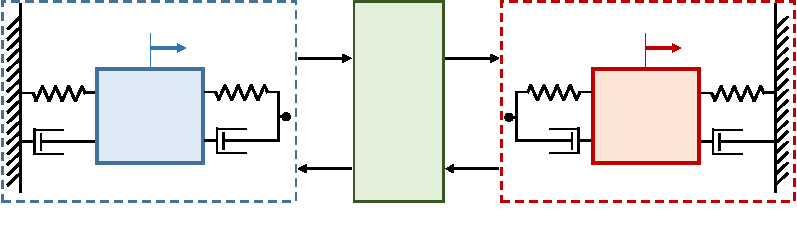
\includegraphics{./fig/LinearOscillatorCosimSS.pdf}};
		
		% Text
		\node[align=center, color = figureBlue] 	at (-42mm, 0mm) {$m_1$};
		\node[align=center, color = figureRed] 		at ( 42mm, 0mm) {$m_2$};
		\node[align=center, color = figureBlue] 	at (-37mm, 14.5mm) {$x_1$};
		\node[align=center, color = figureRed] 		at (47mm, 14.5mm) {$x_2$};
		
		\node[align=center, color = black] 			at (-26mm, 8.5mm) {$k_{\rm c}$};
		\node[align=center, color = black] 			at (-26mm, -8.7mm) {$c_{\rm c}$};
		\node[align=center, color = black] 			at (26mm, 8.5mm) {$k_{\rm c}$};
		\node[align=center, color = black] 			at (26mm, -8.7mm) {$c_{\rm c}$};
		\node[align=center, color = black] 			at (-58mm, 8.5mm) {$k_1$};
		\node[align=center, color = black] 			at (-58mm, -8.7mm) {$c_1$};
		\node[align=center, color = black] 			at (58mm, 8.5mm) {$k_2$};
		\node[align=center, color = black] 			at (58mm, -8.7mm) {$c_2$};
		
		\node[align=center, color=black] 			at (-12.5mm, 13.5mm) {$\eta^{\rm c}_1$};
		\node[align=center, color=black] 			at (12.5mm, 13.5mm) {$\eta^{\rm c}_2$};
		\node[align=center, color=black] 			at (-12.5mm, -13.1mm) {$\xi^{\rm c}_1$};
		\node[align=center, color=black] 			at (12.5mm, -13.1mm) {$\xi^{\rm c}_2$};
		
		\node[align=center, color = figureGreen] 	at (-12mm, 0mm) {$H_1$};
		\node[align=center, color = figureGreen] 	at (12mm, 0mm) {$H_2$};
		
		\node[align=center, color = figureBlue] 	at (-42mm, -19mm) {Subsystem $\mathcal{M}_1$};
		\node[align=center, color = figureRed] 		at (42.5mm, -19mm) {Subsystem $\mathcal{M}_2$};
		
		\node[align=center, color = figureGreen] 	at (0mm, -19mm) {Manager};
		
	\end{tikzpicture}
	\caption{The linear oscillator arranged following a displacement-displacement coupling scheme}
	\label{fig:LinearOscillatorCosim2}
\end{figure}

In this co-simulation configuration, none of the subsystems has direct feed-through.
Subsystem output is part of the state in both cases and can be evaluated without knowledge of the  input at any time.
Accordingly, input extrapolation is not necessary with this configuration.


% -----------------------------------------------------------------------------------------------
\subsection{Force-force co-simulation}
\label{ForceForce}

It is also possible to perform the evaluation of the coupling force outside the subsystems, for instance in the co-simulation manager.
In this case, the subsystems would provide information about their position and velocity to the manager, and would receive the coupling force as input, as shown in Fig.~\ref{fig:LinearOscillatorCosim3}.

\begin{figure}[ht]
	\centering
	\begin{tikzpicture}
		
		% Colors
		\definecolor{figureBlue}{RGB}{65,113,156};
		\definecolor{figureRed}{RGB}{192,0,0};
		\definecolor{figureGreen}{RGB}{56,87,35};
		
		% Figure Drawing
		\node at (0,0) {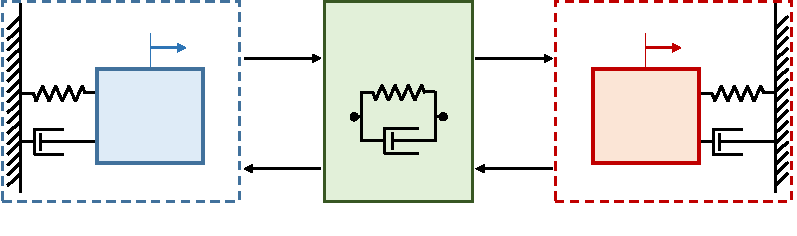
\includegraphics{./fig/LinearOscillatorCosimFF.pdf}};
		
		% Text
		\node[align=center, color = figureBlue] 	at (-42mm, 0mm) {$m_1$};
		\node[align=center, color = figureRed] 		at ( 42mm, 0mm) {$m_2$};
		\node[align=center, color = figureBlue] 	at (-37mm, 14.5mm) {$x_1$};
		\node[align=center, color = figureRed] 		at (47mm, 14.5mm) {$x_2$};
		
		\node[align=center, color = black] 			at (0mm, 8.5mm) {$k_{\rm c}$};
		\node[align=center, color = black] 			at (0mm, -8.7mm) {$c_{\rm c}$};
		\node[align=center, color = black] 			at (-58mm, 8.5mm) {$k_1$};
		\node[align=center, color = black] 			at (-58mm, -8.7mm) {$c_1$};
		\node[align=center, color = black] 			at (58mm, 8.5mm) {$k_2$};
		\node[align=center, color = black] 			at (58mm, -8.7mm) {$c_2$};
		
		\node[align=center, color=black] 			at (-20mm, 13.5mm) {$\eta^{\mathrm c}_1$};
		\node[align=center, color=black] 			at (20mm, 13.5mm) {$f_2^{\mathrm c}$};
		\node[align=center, color=black] 			at (-20mm, -13.1mm) {$f_1^{\mathrm c}$};
		\node[align=center, color=black] 			at (20mm, -13.1mm) {$\xi^{\mathrm c}_2$};
		
		\node[align=center, color = figureGreen] 	at (-20mm, 0mm) {$H_1$};
		\node[align=center, color = figureGreen] 	at (20mm, 0mm) {$H_2$};
		
		\node[align=center, color = figureBlue] 	at (-42mm, -19mm) {Subsystem $\mathcal{M}_1$};
		\node[align=center, color = figureRed] 		at (42.5mm, -19mm) {Subsystem $\mathcal{M}_2$};
		
		\node[align=center, color = figureGreen] 	at (0mm, -19mm) {Manager};
		
	\end{tikzpicture}
	\caption{The linear oscillator arranged following a force-force coupling scheme}
	\label{fig:LinearOscillatorCosim3}
\end{figure}

In this case, the information about the stiffness and damping properties of the coupling interface must be available to the co-simulation manager.
The scheme is similar to the displacement-displacement one, in the sense that the subsystems are free from direct feed-through. 
In fact, for single-rate co-simulation schemes, both coupling approaches are equivalent.
The need to perform input extrapolation in the multi-rate case introduces differences between their results, though.


% _______________________________________________________________________________________________
\section{Simulation}
\label{Simulation}

A 10-s simulation of the system motion, starting from the initial configuration and velocity, in the absence of externally applied forces, is the simulation considered in the definition of this benchmark problem.

For case 1 in Table~\ref{tab:systemParameters} the system is conservative, and so its mechanical energy should remain constant during motion.

% _______________________________________________________________________________________________
\pagebreak
\pagestyle{bib}
\bibliography{./cosimBenchmark}

\end{document}	
